\documentclass[11pt,a4paper]{article}

\usepackage[pdftex]{graphicx}
\usepackage[cmex10]{amsmath}
\usepackage[usenames,dvipsnames]{color}
\usepackage{xspace}
\usepackage{fullpage}
\usepackage{tikz}
\usepackage{pgfplots}
\usepackage{pgfplotstable}
\usepackage{textcomp}
\usepackage{multirow}
\usetikzlibrary{shapes,arrows}
\usetikzlibrary{pgfplots.groupplots}
\usepackage{url}
\usepackage{listings}
\usepackage{framed}

\newcommand{\todo}[1]{\textbf{\textcolor{Blue}{TODO: #1}}}
\newcommand{\hilight}[1]{\textit{\textcolor{Red}{#1}}}
\newcommand{\lst}[1]{\lstinline!#1!}
\newcommand{\fig}[1]{Fig.~\ref{#1}}
\newcommand{\eq}[1]{(\ref{#1})}
\newcommand{\ap}[1]{Appendix~\ref{#1}}
\newcommand{\tbl}[1]{Tbl.~\ref{#1}}
\newcommand{\file}[1]{\lstinline[basicstyle=\normalsize,]!#1!}
\newcommand{\pder}[2]{\frac{\partial{#1}}{\partial{#2}}}
\newcommand{\neuron}{CoreNeuron\xspace}
\newcommand{\dx}{{\Delta x}}
\newcommand{\dt}{{\Delta t}}
\newcommand{\at}[1]{{#1}_{i}}
\newcommand{\atplus}[1]{{#1}_{i+1}}
\newcommand{\atminus}[1]{{#1}_{i-1}}
\newcommand{\atplushalf}[1]{{#1}_{i+\frac{1}{2}}}
\newcommand{\atminushalf}[1]{{#1}_{i-\frac{1}{2}}}
\newcommand{\vv}[1]{\mathbf{#1}}
\newcommand{\att}[1]{{#1}^{n}}
\newcommand{\attplus}[1]{{#1}^{n+1}}
\newcommand{\attplushalf}[1]{{#1}^{n+\frac{1}{2}}}
\newcommand{\hoc}{\lst{.hoc}\xspace}

\lstdefinelanguage{julia}
{
    morekeywords = {
        if, elseif, else,
        for, while, end, in, using, local,
        type, function, return, yieldto, try, catch, error, throw, begin, quote,
        Int, Int32, Int64, Float, Float32, Float64, Array
    },
    sensitive = true,
    morecomment=[l]\#,
    morestring=[b]",
    morestring=[b]',
    moredelim=*[directive]@,
    moredirectives={assert, time, eval} % macros
}[keywords,comments,strings,directives]


\lstset{
    language=[ANSI]C++,
    %numbers=left,
    basicstyle=\small\ttfamily,
    identifierstyle=\color{Blue}\small\ttfamily,
    keywordstyle=\color{Red}\small\ttfamily\bf,
    commentstyle=\color{OliveGreen}\small\ttfamily,
    breaklines=true
}
\lstset{
    emph={pw_stop_collector,
          pw_start_collector,
          pw_new_collector,
          pw_print_table
    },
    emphstyle={\color{Bittersweet}\bfseries\normalsize}
}

\definecolor{shadecolor}{rgb}{0.8,0.8,0.8}

\begin{document}

% title and cover page
\title{\neuron Overview}
\author{Ben Cumming\\CSCS -- Swiss National Supercomputing Center}
\date{\today}
\maketitle

% abstract
\abstract{
This document presents an overview of the \neuron code that was released as part of the PCP process for the Human Brain Project in July 2014. The analysis focuses on the structure of the code that has the highest computational overheads.

More detailed analysis of the algorithms themselves, and important parts of the code like spike communication, that do not contribute meaniningfully to the time to solution are not considered for analysis. For now I will focus on just the computationally intensive parts of the code.

Note that this analysis is based on an early version of the \neuron code, and that different algorithms (e.g. modelling plasticity) may significantly increase the importance of parts of the application not yet considered here.
}

%%%%%%%%%%%%%%%%%%%%%%%%%%%%%%%%%%%%%%%%%%%%%%%%%%%%%%%%%%%%%%
\section{What is \neuron?}
%%%%%%%%%%%%%%%%%%%%%%%%%%%%%%%%%%%%%%%%%%%%%%%%%%%%%%%%%%%%%%
The version of \neuron that was released for the PCP is derived directly from \emph{Bluron}, a flavour of \emph{Neuron} maintained by the Blue Brain Project (BBP) group at EPFL. \neuron is derived directly in the sense that it is a subset of the features and corresponding code from \emph{Bluron}. The code has been modified as much as needed to remove it from the larger \emph{Bluron} infrastructure, and reduce the memory footprint of the code.

Note that \emph{Bluron} refers to the \emph{Neuron} plus the \hoc files used to define the models used in the BBP group. The computational back end is identical for both \emph{Bluron} and \emph{Neuron}. \hilight{Correct me if this is wrong.}

%%%%%%%%%%%%%%%%%%%%%%%%%%%%%%%%%%%%%%%%%%%%%%%%%%%%%%%%%%%%%%
\section{The Code}
The code in its current form is a mixture of C and C++.

It must be noted that the code base is currently very challenging to understand and benchmark. It is derived directly from the Bluron/Neuron code base, which has grown organically over a period of more tha 20 years. As such there are very many opportunities to simplify and improve the code using modern programming languages and development techniqies.

To use both CPUs and accelerators (e.g. GPU and MIC) effectively, parts of the code will have to be refactored, or rewritten significantly. Rewriting will be challenging, given the difficulty of understanding the current code, which is a prerequisite for rewriting the code. Developing documentation of the algorithms as they are currently implemented is essential if the code is to be refactored.

From early work with the code base, the majority of wall time for the example circuits release for the PCP is spent in a relatively small set of code: the \lst{nrnoc} solver implementation, and the mechanisms defined in \lst{/mecb/cfiles}. The code in its current form might be difficult to reason about, however the algorithms themselves are relatively straightfoward.

An aim of this report is as a first attempt at describing the algorithms clearly, to make it possible to reason about how them without getting distracted by implementation details. To assist in this, many of the algorithms are presented in a pseudo-language similar to \emph{Julia}\footnote{See the website: \file{julialang.org}}, which should be familiar to users familiar with \emph{Matlab}.

%-------------------------------------------------------------
\subsection{Code Issues}
%-------------------------------------------------------------
Some of the anti-patterns that make understanding the code difficult are:
\begin{itemize}
    \item
        There are many global variables. With many static symbols used for scoping within a translation units, which makes understanding where variables are defined and used challenging.
    \item
        The use of preprocessor \lst{#define} makes the code very difficult to reason about. Many variable names are redefined, which obscures the meaning of the code. There are also many ``magic numbers'' that are defined on differently in different translation units.
    \item
        The C++ code uses new and delete keywords, sometimes forgetting to delete. Should use static arrays or STL containers depending on needs.
    \item
        overly complicated data structures that make it very difficult for both humans and compilers to reason about the code. As a result there are a lot of lost opportunities for optimization for the compiler.
    \item
        Poor (non-existant in places) comments and naming of variables.
\end{itemize}

%-------------------------------------------------------------
\subsection{Code Layout}
%-------------------------------------------------------------
The source code is packaged in a file \lst{CoreBluron.tar.gz}, which has the directory structure in \fig{fig:DirectoryStructure}.
In terms of time to solution, functions defined in \lst{mech/cfiles} dominate. These are called from the solver routines in \lst{nrnoc}, which implements the core computation, and is the focus of the analysis here.

\begin{figure}[tp!]
%---------------------------
\fbox{ \parbox{\textwidth} {

\begin{itemize}
    %%%%%%%%%%%%%%%%%%%%%%%%%%%%%%%%%%%%%%%%%
    \item \textbf{nrniv}
    \begin{itemize}
        \item C and C++ (11,470 lines).
        \item The \neuron driver: \lst{main()} is in \lst{main1.cpp}.
    \end{itemize}

    %%%%%%%%%%%%%%%%%%%%%%%%%%%%%%%%%%%%%%%%%
    \item \textbf{nrnoc}
    \begin{itemize}
        \item C (2,889 lines).
        \item The \neuron ``engine''
        \begin{itemize}
            \item storage
            \item solvers
            \item time stepping
        \end{itemize}
    \end{itemize}

    %%%%%%%%%%%%%%%%%%%%%%%%%%%%%%%%%%%%%%%%%
    \item \textbf{mech/cfiles}
    \begin{itemize}
        \item C (11,301 lines).
        \item Definitions of all the mechanisms.
        \item generated from \hoc files by Neuron.
        \item the generated code is very messy (use \lst{clang-format} to make things bearable)
    \end{itemize}

    %%%%%%%%%%%%%%%%%%%%%%%%%%%%%%%%%%%%%%%%%
    \item \textbf{nrnmpi}
    \begin{itemize}
        \item C (1,096 lines).
        \item Wrappers around MPI routines.
        \item Spike exchange implementation.
        \item Global variables that store MPI state.
    \end{itemize}

    %%%%%%%%%%%%%%%%%%%%%%%%%%%%%%%%%%%%%%%%%
    \item \textbf{utils}
    \begin{itemize}
        \item C++ (4,494 lines)
        \item Random number generators
    \end{itemize}
\end{itemize}

}}
%---------------------------

\caption{Overview of the directory structure for the source code. There are a total of 31,250 lines of code (including white space and comments).}
\label{fig:DirectoryStructure}

\end{figure}

%%%%%%%%%%%%%%%%%%%%%%%%%%%%%%%%%%%%%%%%%%%%%%%%%%%%%%%%%%%%%%
\subsection{Building}
%%%%%%%%%%%%%%%%%%%%%%%%%%%%%%%%%%%%%%%%%%%%%%%%%%%%%%%%%%%%%%
The code was built on Cray XC-30 system Piz Daint at CSCS with minimal fuss using the GNU toolchain.
The Cray compiler toolchain had problems that are not insurmountable, but they would require a lot of tinkering with the \emph{Buildyard}\footnote{\file{github.com/Eyescale/Buildyard}} build tool used by \neuron.

The Buildyard uses cmake, with a custom set of cmake modules developed by BBP (the BuildYard modules). Many of these modules are not required by \neuron, and configuration can be sped up significantly by removing them (for example the C++11 tests). The cmake configuration attempts to determine the version of the Cray compiler by passing a flag that the compiler doesn't recognise, causing the configuration to exit.

%%%%%%%%%%%%%%%%%%%%%%%%%%%%%%%%%%%%%%%%%%%%%%%%%%%%%%%%%%%%%%
\subsection{Datasets}
%%%%%%%%%%%%%%%%%%%%%%%%%%%%%%%%%%%%%%%%%%%%%%%%%%%%%%%%%%%%%%
There are two data sets provided with the PCP benchmark code:
\begin{itemize}
    \item \textbf{TEST1\_CACHE} A network small enough to fit into Cache of one rack of BG/Q. Has size of 2.5G on disk.
    \item \textbf{TEST2\_DRAM} A much larger network (size 4.5T on disk), that fits in DRAM of one rack of BG/Q.
\end{itemize}

%%%%%%%%%%%%%%%%%%%%%%%%%%%%%%%%%%%%%%%%%%%%%%%%%%%%%%%%%%%%%%



\section{Code Walkthrough}
In this section an will look at how the main time-stepping algorithm, which accounts for nearly all the time to solution, is implemented. However, before looking at the time step implementation, a short description of all of the main stages of the simulation is presented to put the time stepping code in context.
%%%%%%%%%%%%%%%%%%%%%%%%%%%%%%%%%%%%%%%%%%%%%%%%%%%%%%%%%%%%%%
\subsection{Overview of Main}
%%%%%%%%%%%%%%%%%%%%%%%%%%%%%%%%%%%%%%%%%%%%%%%%%%%%%%%%%%%%%%
The driver code is in \file{nrniv/main1.cpp}. From the breakdown of the wall time for the TEST2 data set in \tbl{tbl:wallmain} it is apparent that from a computational point of view, the only component of importance is the time stepping/sover portion of the program in \lst{BBS_netpar_solve}, which takes 99.8\% of time to solution.

Nevertheless, I will breifly describe the other steps performed in the main driver:
\begin{enumerate}
\item \lst{mk_mech}\\
The mechanisms are configured. A text file with a tuple for each mechanism (name, unique index, parameter count, type,  etc \dots) is scanned. This text file is generated when the cell group files are generated by HBPNeuron. This information provides a bridge between the runtime and the mechanisms implemented using the Neuron \hoc language.
\item \lst{mk_netcvode}\\
    Creates a new \lst{NetCvode} object (see \file{nrnoc/netcvod.h/cpp}). This sets up the priority queue use to send and deliver spiking events.
\item \lst{nrn_setup}\\
    Before calling \lst{nrn_setup}, the configuration file \file{files.dat} is read to see how many and which cells are to be loaded for simulation. The cells are assigned in a round-robin fashion between the MPI ranks. Then \lst{nrn_setup} is called with a list of cell ids, to load the cell data from disk.
\item \lst{BBS_netpar_mindelay} and \lst{mk_spikevec_buffer}\\
    The mindelay and spike buffer size are configured. All neuron cells can be integrated-in-time independently for the \emph{minimum network connection delay}, i.e. spikes do not have to be delivered in the interval in which they were generated. These interval boundaries are used as synchronization points.
\item \lst{BBS_netpar_solve} \\
    The time stepping code. The focus of this report.
\item \lst{output_spikes} \\
    Write spike information to disk.
\end{enumerate}

%-------------------------------------------------------------------------------
\begin{table}[htp!]
    \centering
%-------------------------------------------------------------------------------
\begin{tabular}{lrr}
\hline
section                    &    wall time (s) & contribution \% \\
\hline
\lst{mk_mech}            &    0.01   &    0.0\\
\lst{mk_netcvode}        &    0.00   &    0.0\\
\lst{nrn_setup}          &    0.69   &    0.2\\
mindelay/spike buffer      &    0.15   &    0.0\\
\lst{BBS_netpar_solve}   &    388.93 &   99.8\\
\lst{output_spikes}      &    0.01   &    0.0\\
\hline
\end{tabular}
%-------------------------------------------------------------------------------
\label{tbl:wallmain}
\caption{Breakdown of wall time for TEST2 data set running on one node of Piz Daint, with 1 cell per core.}
\end{table}
%-------------------------------------------------------------------------------

%%%%%%%%%%%%%%%%%%%%%%%%%%%%%%%%%%%%%%%%%%%%%%%%%%%%%%%%%%%%%%
\subsection{Drilling Down to The Time Step}
%%%%%%%%%%%%%%%%%%%%%%%%%%%%%%%%%%%%%%%%%%%%%%%%%%%%%%%%%%%%%%
The time stepping and all computation associated with it are performed in the \lst{BBS_netpar_solve} routine. A backtrace of the call tree from \lst{BBS_netpar_solve} to \lst{nrn_fixed_step_thread}, where 100\% of the computation is performed, is shown in \fig{fig:bbsnetpar}. The exact role played by each of these routines is not important now: some of them , and others are wrappers for passing cell groups to a pthread to separate integration (see \sect{sec:data} for more information about cell groups and threads). It is the integration of individual cell groups inside the lowest level function, \lst{nrn_fixed_step_thread} that interests us.

\begin{figure}[htp!]
\centering
\includegraphics[width=\textwidth]{./images/bbs_netpar_solve.pdf}
\caption{backtrace to the main computational routine.}
\label{fig:bbsnetpar}
\end{figure}

Each MPI rank has a set of cells assigned to it in a round robin fashion during the initialization phase (in the call to \lst{nrn_setup} in \lst{main}).
The cells are packaged together into \emph{cell groups}, with one cell group per intput file. The selection of cells in a cell group is chosen when the input files are generated to improve load balancing (static load balancing).
For more information, see \sect{sec:data}.

%The cells are then assigned to a \lst{NrnThread} on each MPI rank. An abreviated definition of is given in \fig{lst:NrnThread}

%\begin{figure}
%\begin{shaded}
%\begin{lstlisting}
%struct NrnThread {
%  // list of mechanisms
%  NrnThreadMembList *tml;
%
%  int ncell;        // number of cells
%  int end;          // number of segments
%  double *_data;    // data for all segment values
%  ...               // other data fields
%
%  // arrays holding matrix system values
%  double *_actual_rhs;
%  double *_actual_d;
%  double *_actual_a;
%  ...
%  // area of each segment
%  double *_actual_area;
%  // parent index of segments
%  int *_v_parent_index;
%};
%\end{lstlisting}
%\end{shaded}
%\label{lst:NrnThread}
%\caption{The definition of the \lst{NrnThread} data type from \file{nrnoc/multicore.h}. Note that many data members have been removed, with just some fields of interest included.}
%\end{figure}

%*******************************************************************************
\begin{figure}[htp!]
\centering
\includegraphics[width=\textwidth]{./images/calltree.pdf}
\caption{Calltree and percentage of wall time contribution for the main computational algorithm. Branches marked in blue indicate a significant contribution to wall time.}
\label{fig:calltree}
\end{figure}
%*******************************************************************************



\subsection{The Algorithm}
The call to \lst{nrn_fixed_step_thread()} implements a single time step for the set of cells on a thread, and accounts for over 99\% of all wall time. When discussing \emph{the algorithm} here, the focus is on the algorithm as implemented: with a higher level mathematical description of the algorithm proper where required to help understanding.

%%%%%%%%%%%%%%%%%%%%%%%%%%%%%%%%%%%%%%%%%%%%%%%%%%%%%%%%%%%%%%%%%%
\subsubsection{Spatial Discretization and Cable Equation}
%%%%%%%%%%%%%%%%%%%%%%%%%%%%%%%%%%%%%%%%%%%%%%%%%%%%%%%%%%%%%%%%%%
We first look at the spatial discretization of the partial differential equation (PDE) in \neuron. We consider a partial differential equation in one dimension with the general form
\begin{equation}
     C\pder{V}{t} + I = f \pder{}{x} \left( g\pder{V}{x} \right)
\end{equation}
where $f$ and $g$ are functions of the spatial dimension $x$ (they are functions of \emph{cable radius} in this model). The value of $I$ is dependent on the voltage $V$.

The spatial and temporal discretization used in Neuron is finite difference with a Crank Nicholson time stepping scheme. The time stepping scheme has an odd form, that differs slightly from the scheme presented here. However, the exposition here adequately characterizes the code.

\emph{Finite Difference Methods in Heat Transfer, Second Edition} By Necati Ozisik (1994) gives the following finite difference discretization
\begin{align}
    \dx \left(\at{C} \frac{\attplus{\at{V}} - \att{\at{V}}}{\dt} + \attplushalf{\at{I}} \right)
    &=\nonumber \\
    & \at{f} \theta
            \left[
                \atminushalf{g} \frac{\atminus{V}^{n+1}-\at{V}^{n+1}}{\dx}
              + \atplushalf{g}  \frac{\atplus{V}^{n+1}-\at{V}^{n+1}}{\dx}
            \right] \nonumber \\
            + & \at{f} (1-\theta)
            \left[
                \atminushalf{g} \frac{\atminus{V}^{n}-\at{V}^{n}}{\dx}
              + \atplushalf{g}  \frac{\atplus{V}^{n}-\at{V}^{n}}{\dx}
            \right]
        \label{eq:cableDiscretization}
\end{align}

where the parameter $\theta$ can be used to determine the time stepping scheme ($\theta=0$ explicit, $\theta=1$ implicit, $\theta=1/2$ Crank-Nicholson).

Note that the quantity $I$ depends on the value of $V$. These values have to be evaluated to form coefficients in the linear system that is to solved at each time step. The approach taken by Neuron is the evaluate them at a half time step value at $t+\dt/2$, denoted $\attplushalf{\at{I}}$, by implicitly solving for a half step, then performing an explicit half step.

With a Crank Nicholson time stepping scheme, i.e. $\theta=1/2$, the terms on the right hand side of \eq{eq:cableDiscretization} simplify to
\begin{align}
        \frac{\at{f}}{2}
        &\left\{
            \left[
                \atminushalf{g} \frac{\atminus{V}^{n+1}-\at{V}^{n+1}}{\dx}
              + \atplushalf{g}  \frac{\atplus{V}^{n+1}-\at{V}^{n+1}}{\dx}
            \right]
        \right. \nonumber \\
        +
        &\left.
            \left[
                \atminushalf{g} \frac{\atminus{V}^{n}-\at{V}^{n}}{\dx}
              + \atplushalf{g}  \frac{\atplus{V}^{n}-\at{V}^{n}}{\dx}
            \right]
        \right\} \label{eq:crankNichRHS}
\end{align}

Substituting the spatial discretization in~\eq{eq:crankNichRHS} into~\eq{eq:cableDiscretization} and rearranging gives a tri-diagonal linear system with the form
\begin{equation}
    \at{a} \atplus{V}^{n+1} + \at{d} \at{V}^{n+1} + \at{b} \atminus{V}^{n+1} = \at{r}
\end{equation}
where the diagonals in the matrix are defined
\begin{align}
    \at{a}  &=  -\frac{\at{f}\atplushalf{g}}{2\dx^2} \\
    \at{b}  &=  -\frac{\at{f}\atminushalf{g}}{2\dx^2} \\
    \at{d}  &=  \frac{\at{C}}{\dt} + \frac{f}{2\dx^2}\left[\atminushalf{g}+\atplushalf{g}\right] \nonumber\\
            &=  \frac{\at{C}}{\dt} - ( \at{a} + \at{b} ) \\
\intertext{and}
    \at{r}  &=  \frac{\at{C}}{\dt} \at{V}^n - \at{I} + \frac{\at{f}}{2\dx^2}
                    \left[
                        \atminushalf{g} \left( \atminus{V}^{n} - \at{V}^{n} \right)
                        +
                        \atplushalf{g}  \left( \atplus{V}^{n}  - \at{V}^{n} \right)
                    \right] \nonumber\\
            &=  \frac{\at{C}}{\dt} \at{V}^n
                - \at{I}
                - \at{a} \left( \atminus{V}^{n} - \at{V}^{n} \right)
                - \at{b} \left( \atplus{V}^{n}  - \at{V}^{n} \right)
\end{align}

It is important to note that the coefficients in the linear system are constant in time. In practice the off-diagonal entries in $\vv{a}$ and $\vv{b}$ are computed once at start up. The values on the diagonal, i.e. those in $\vv{d}$ are overwritten when solving the linear system using Thomas' algorithm. They are reconstructed using the values stored in $\vv{a}$ and $\vv{b}$
%%%%%%%%%%%%%%%%%%%%%%%%%%%%%%%%%%%%%%%%%%%%%%%%%%%%%%%%%%%%%%
\subsubsection{Not quite one-dimensional: trees \& branching}
%%%%%%%%%%%%%%%%%%%%%%%%%%%%%%%%%%%%%%%%%%%%%%%%%%%%%%%%%%%%%%
In the previous subsection a one-dimensional model and it's discretization were described, while ignoring the impact of boundary conditions. We will now extend this description to handle branching, whereby the domain is composed of a series of one-dimensional \emph{sections}, that are joined at branch points to form a tree.

A small tree structure is illustrated in \fig{fig:tree}(a). It is important to note that the graph formed by the branching sections is a true tree, i.e. it has no circuits (once a section has branched, the branches can not ``rejoin'').

\begin{figure}[htp!]
\centering
\includegraphics[width=0.6\textwidth]{./images/tree.pdf}
\\{\normalsize (a)}\\
\includegraphics[width=\textwidth]{./images/discrete_a.pdf}
\includegraphics[width=\textwidth]{./images/discrete_b.pdf}
\includegraphics[width=\textwidth]{./images/discrete_c.pdf}
\includegraphics[width=\textwidth]{./images/discrete_d.pdf}
\includegraphics[width=\textwidth]{./images/discrete.pdf}
\\{\normalsize (b)}
\caption{Numbering of nodes and edges for Hines algorithm. (a) The high level branch and connection numbering scheme, with the branch nodes and sections numbered; (b) the numbering of individual nodes in the fully discretized domain with 5 segments per section.}
\label{fig:tree}
\end{figure}

Some terms used in discussing the tree structure in \fig{fig:tree} are:
\begin{itemize}
        \item \textbf{section} a branch in the tree structure, which corresponds to the one-dimensional line segmant between branch points. These are numbered $s*$ in \fig{fig:tree}(a).
        \item \textbf{branch} same definition as section.
        \item \textbf{node} a point in the spatial discretization. These are numbered in \fig{fig:tree}(b).
        \item \textbf{branch node} a node where two branches join. These are the blue points denoted $n*$ \fig{fig:tree}(a).
        \item \textbf{terminal branch} a branch that is one node that has one end that is connected to no other branches.
        \item \textbf{terminal node} a node that lies at the end of a branch that connects to no other branches. These correspond to $n1$, $n4$, $n5$ and $n6$ in \fig{fig:tree}(a).
\end{itemize}

The first step of the spatial discretixation is to discretize each one-dimensional section. Then the nodes are numbered using a scheme that gives the matrix a sparsity structure that allows the linear system to be solved in linear time, equivalent to Thomas algorithm.

The numbering scheme is as follows
\begin{enumerate}
\item
    A \emph{terminal branch} of the tree is selected, and its nodes are numbered with the terminal node last.
    The node numbered 1 is referred to as the \emph{root node} of the tree, and is shown in red in \fig{fig:tree}(b).
\item
    The tree is then traversed, with the nodes on each individual edge numbered such that the node index is higher for nodes further from the root. The sequence of steps illustrated in \fig{fig:tree}(b) shows the numbering applied in this manner as each branch of the tree is visited.
\end{enumerate}
A data-structure and algorithm for building the tree in \fig{fig:tree} are shown in \ap{appendix:treesource}. The source code for this was used to generate the images in this document.

The tree and it's corresponding matrix representation have the following properties:
\begin{itemize}
\item
    Every node has exactly one parent, except for the root node. In all cases the index of the parent $p_i$ of node $i$ is less than the index of the node, i.e. $p_i<i,~\forall\,i\in\left\{1,2,\dots,N\right\}$, where $N$ is the total number of nodes.
\item
    Non-terminal nodes have at least one child, i.e. nodes that have it as a parent, with branch nodes having one child for each branch in their subtree.
\item
    It is only necessary to store the parent indexes, the $p_i$ values, for each node in the tree.
\item
    The sparsity pattern of the linear system associated with this numbering has the following properties:
    \begin{itemize}
    \item
        The sparsity pattern is symmetric.
    \item
        the diagonal values are all nonzero.
    \item
        their is exactly one off diagonal value in each row of the lower triangle at $a_{ik}$, where $k=p_i$.
    \item
        their is exactly one off diagonal value in each column of the upper triangle at $a_{ki}$, where $k=p_i$.
    \end{itemize}
\item
    The sparsity pattern for the network in \fig{fig:tree}(b) is shown in \fig{fig:sparsity}. The pattern matrix was generated from the code in \ap{appendix:treesource}.
\item
    A matrix with this sparsity pattern can be stored with three vectores, $\vv{a}$, $\vv{b}$ and $\vv{c}$, where:
    \begin{align}
        a_i &= A_{ki} \\
        b_i &= A_{ik} \\
        d_i &= A_{ii}
    \end{align}
    where $k=p_i$.
\end{itemize}

\begin{figure}[htp!]
\centering
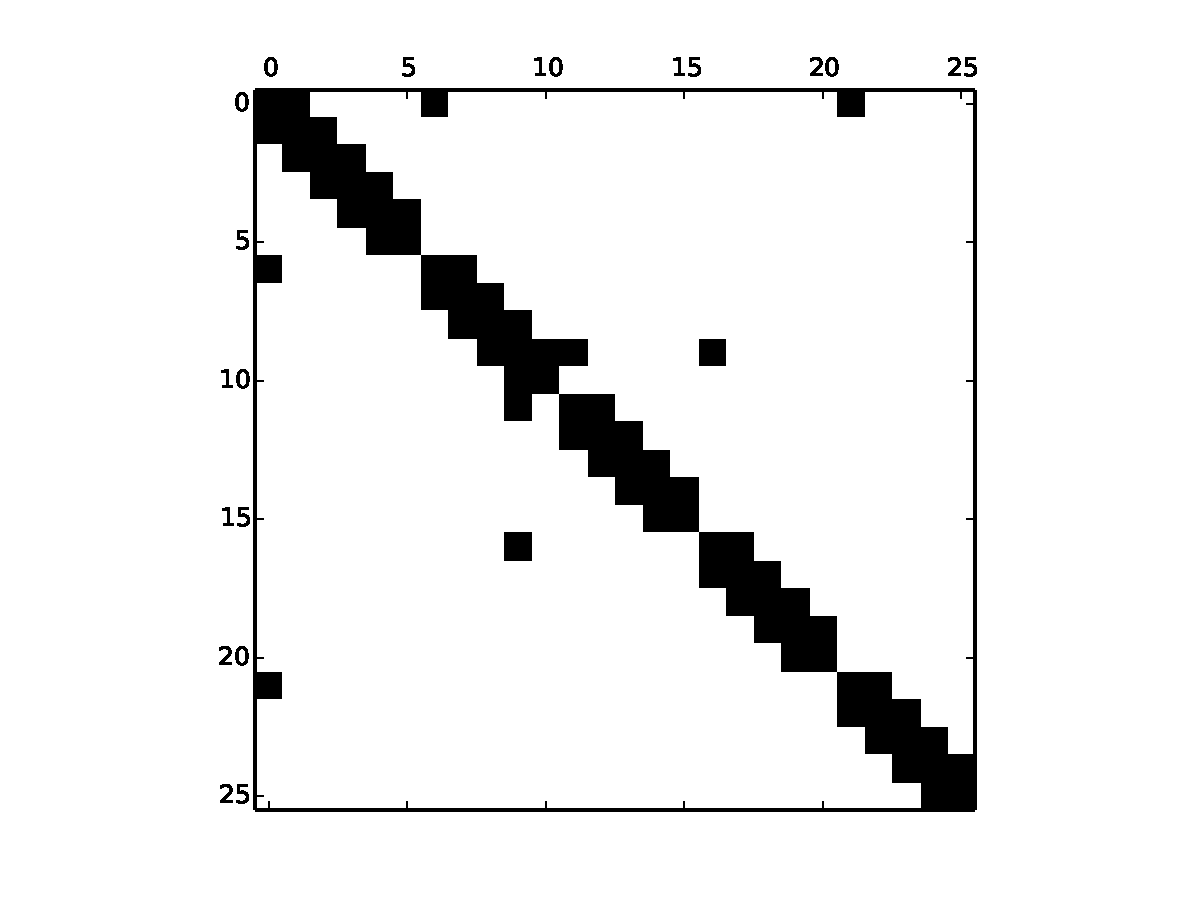
\includegraphics[width=0.5\textwidth]{./images/sparsity.pdf}
\caption{Sparsity pattern of the matrix corresponding to the tree numbering in \fig{fig:tree}.}
\label{fig:sparsity}
\end{figure}


The linear systems that arise from the discretization of the branching cable equation can be solved very efficiently, in linear $O(N)$ time, using an algorithm that is equivalent to the Thomas algorithm for solving tri-diagonal systems. This algorithm, called Hines algorithm, proceeds by eliminating the nonzero entries in the upper triangle of $A$. Recall the matrix property that there is only one non-zero value in each column of the upper triangle
 at $A_{ki}$, which is stored in $a_i$.
\begin{equation}
\left(
        \begin{array}{ccc}
            A_{kk} & \dots      & A_{ki} \\
        \vdots     & \ddots     & \mathbf{0} \\
            A_{ik} & \mathbf{0} & A_{ii}
        \end{array}
\right)
\text{which is stored as:}
\left(
        \begin{array}{ccc}
            d_k & \dots      & a_i \\
        \vdots  & \ddots     & \mathbf{0} \\
            b_i & \mathbf{0} & d_i
        \end{array}
\right)
\end{equation}
The value $a_i$ and can be zeroed out with a row operation
\begin{equation*}
    \text{row}_k \leftarrow \text{row}_k - a_i/d_i\cdot\text{row}_i.
\end{equation*}
In practice the value of $a_i$ is not changed, and only the diagonal entry has to be modified
\begin{equation*}
d_k \leftarrow d_k - a_i/d_i\cdot b_i.
\end{equation*}
The forward substitution is then used to determine the solution. The forward and backward substitution are implemented in Julia in \ap{appendix:hinessource}.




\subsection{Implementation of a time step}
In this section the implementation of the code that forms and solves the matrix, which accounts for 99\% of the time to solution will be described. The algorithm themselves are quite simple, however their implementation is very difficult to understand. To make it easier to understand to understand implementation, the core routines have been rewritten in a high-level pseudo code similar to Julia.

An example of the pseudo code represents the following C code
\begin{shaded}
\begin{lstlisting} [breaklines=true]
for (tml = _nt->tml; tml; tml = tml->next)
  if (memb_func[tml->index].current) {
    mod_f_t s = memb_func[tml->index].current;
    (*s)(_nt, tml->ml, tml->index);
  }
\end{lstlisting}
\end{shaded}
\noindent as
\begin{shaded}
\begin{lstlisting} [language=julia,breaklines=true]
for mechanism in thread.mechanisms
  mechanism.current(thread, mechanism.data)
end
\end{lstlisting}
\end{shaded}
\noindent There is a trade-off, whereby idiomatic Julia code would look like the following, but it is kept in the form above to more closely match the data flow in the C code
\begin{shaded}
\begin{lstlisting} [language=julia,breaklines=true]
for mechanism in thread.mechanisms
  current(mechanism)
end
\end{lstlisting}
\end{shaded}
\noindent Not that a similar level of clarity would be possible with well-designed C+11 code.

The inner part of each time step is implemented in the function \lst{nrn_fixed_step_thread()}, in \file{nrnoc/fadvance_core.c}. The routine takes as its argument a pointer to a struct of type \lst{NtnThread}, see \fig{lst:NrnThread}, which holds state relating to a set of cells to be integrated in time.
\begin{shaded}
\lstinputlisting [language=julia,breaklines=true] {./code/fixed_step_thread.jl}
\end{shaded}

A breakdown of wall time for the steps in \lst{nrn_fixed_step()} is given in \fig{fig:calltree}. Some of the routines listed here have less than 1\% of wall time (including the linear system solve in \lst{nrn_solve_minimal()}), however they are discussed below because they access they have implementation details that will influence the implementation on many-core architectures (e.g. GPU and MIC).

%%%%%%%%%%%%%%%%%%%%%%%%%%%%%%%%%%%%%%%%%%%%%%%%%%%%%%%%%%%%%%
\subsubsection{Building matrix and RHS: \lst{setup_tree_matrix()}}
%%%%%%%%%%%%%%%%%%%%%%%%%%%%%%%%%%%%%%%%%%%%%%%%%%%%%%%%%%%%%%
The function \lst{setup_tree_matrix()} generates the diagonal, the $d_i$ values, and the RHS vector. These tasks are performed in two separate routines, \lst{nrn_lhs()} and \lst{nrn_rhs()}.
\begin{shaded}
\lstinputlisting [language=julia,breaklines=true] {./code/setup_tree_matrix.jl}
\end{shaded}

Points
\begin{itemize}
\item
    The array \lst{p} is an index array containing the parent node indexes.
\item
    The arrays \lst{VEC_*} correspond to the vectors $\vv{a}, \vv{b}, \vv{d}, \vv{v}, \vv{r}$ that define the linear system.
\item
    Each thread has multiple cells, each with their own tree representation. The cells are packed together, with the root node of each cell placed first in the list of all nodes, hence the definition of \lst{child_nodes} excluding indexes $1:ncells$.
\item
    Nearly all (i.e. 99\%) of the time in these two routines is spent in the calls to the \lst{mechanism.current()} and \lst{mechanism.jacob()} routines.
\item
    The matrix updates still must be considered, because there are potential race conditions in a multi-threaded/GPU implementation. For example the statement \lst{VEC_RHS[p[i]] += dv * VEC_A[i]} will lead to a race condition if two threads with the same parent node try to update the RHS vector at the same time.
\end{itemize}

The \lst{mechanism.current()} and \lst{mechanism.jacob()} routines are defined in the \file{/mech/cfiles} path, and are automatically generated from Neuron hoc DSL. \fig{fig:calltree} shows that all of the computational work in the \neuron benchmark used in this report is performed by functions from the hoc layer. The \lst{jacob} functions are also very simple, and all have the same form (I think, there may be some exceptions)
\begin{shaded}
\lstinputlisting [language=julia,breaklines=true] {./code/jacob.jl}
\end{shaded}

The \lst{mechanism.current} calls contribute 45\% of time to solution for the TEST2 benchmark. They are uniquely defined for each mechanism. \hilight{Is it possible to present a few different examples that have all the expected \emph{patterns} in a current implementation?}. A ``representative'' example of a \lst{current} implementation is:
\begin{shaded}
\lstinputlisting [language=julia,breaklines=true] {./code/current.jl}
\end{shaded}

The \lst{nrn_cap_jacob()} function is a very simple, illustrating a common data access pattern whereby a vector (int this case \lst{VEC_D}) is updated according to the parent node if the loop index:
\begin{shaded}
\lstinputlisting [language=julia,breaklines=true] {./code/nrn_cap_jacob.jl}
\end{shaded}

%%%%%%%%%%%%%%%%%%%%%%%%%%%%%%%%%%%%%%%%%%%%%%%%%%%%%%%%%%%%%%
\subsubsection{Solving the linear system: \lst{nrn_solve_minimal()}}
%%%%%%%%%%%%%%%%%%%%%%%%%%%%%%%%%%%%%%%%%%%%%%%%%%%%%%%%%%%%%%
The solution of the linear system using Hines algorithm is straightforward, and is implemented in \file{/nrnoc/solve_core.c}.

\begin{shaded}
\lstinputlisting [language=julia,breaklines=true] {./code/nrn_solve_minimal.jl}
\end{shaded}

%%%%%%%%%%%%%%%%%%%%%%%%%%%%%%%%%%%%%%%%%%%%%%%%%%%%%%%%%%%%%%
\subsubsection{Advancing the solution: \lst{update()}}
%%%%%%%%%%%%%%%%%%%%%%%%%%%%%%%%%%%%%%%%%%%%%%%%%%%%%%%%%%%%%%

These routines have almost no computational overhead, and are included here for completeness.

The solution to the linear system, stored in \lst{VEC_RHS} is actually the delta in solution, that is $\at{\text{RHS}} = \at{V}^{n+1} - \at{V}^{n}$. The \lst{update()} function updates the solution in \lst{VEC_V} by adding the contribution in \lst{VEC_RHS}. The \lst{update()} function is the only part of the \neuron code that successfully vectorizes, because of the stride-one data access pattern in the update.

\hilight{It is not immediately obvious what the purpose of the \lst{second_order_cur()} and \lst{nrn_capacity_current()} routines is}.

\begin{shaded}
\lstinputlisting [language=julia,breaklines=true] {./code/update.jl}
\end{shaded}
%%%%%%%%%%%%%%%%%%%%%%%%%%%%%%%%%%%%%%%%%%%%%%%%%%%%%%%%%%%%%%
\subsubsection{Updating \emph{state}: \lst{nonvint()}}
%%%%%%%%%%%%%%%%%%%%%%%%%%%%%%%%%%%%%%%%%%%%%%%%%%%%%%%%%%%%%%
The \lst{nonvint()} function is a simple lookup of the \lst{state()} function defined for each mechanism. These calls are a significant contribution to computational overheads -- greater than 40\% for the TEST2 benchmark.

\begin{shaded}
\lstinputlisting [language=julia,breaklines=true] {./code/nonvint.jl}
\end{shaded}

The \lst{state()} function implementations are derived from the \file{.hoc} implementation. These have obvious potential for vectorization, because they do not appear to have the ``parent update'' pattern in other loops. However this would require using structore of array (SoA) storage (see the next section). Below is an example of one state update -- note the many exponentials (some of which are redundant)

\begin{shaded}
\lstinputlisting [language=julia,breaklines=true] {./code/state.jl}
\end{shaded}

%%%%%%%%%%%%%%%%%%%%%%%%%%%%%%%%%%%%%%%%%%%%%%%%%%%%%%%%%%%%%%
\subsubsection{Mechanism implementation from .hoc files}
%%%%%%%%%%%%%%%%%%%%%%%%%%%%%%%%%%%%%%%%%%%%%%%%%%%%%%%%%%%%%%
A generic interface for mechanisms is used, with the individual mechanisms defined in \file{/mech/cfils}.

Neuron provides a generic interface for the implementation of user-defined mechanisms.

The majority (98\%) of time is spent in the \lst{current}, \lst{jacob} and \lst{state} routines implemented in these routines.

\todo{description of the poor man's vtable. Mechanism registering.}

\todo{description of AoS storage. Per-thread storage. Access patterns. Possible strategies for SoA.}


\section{Benchmarking}
Here we present preliminary benchmarking results based on the benchmark datasets distributed with the PCP benchmark. The benchmark data is untarred to the paths \file{VENDORS/TEST1_CACHE} and \file{VENDORS/TEST2_DRAM}, which contain data files \file{[0-9]*.dat} that define $2^{14}=16,384$ and $2^{15}=32,768$ individual cells respectively. The number of cells to use in a simulation is set in the first line of the file \file{files.dat}. The cells are assigned to individual MPI ranks in a round-robin fashion, e.g. 32 files with 8 MPI ranks will assign $32/8=4$ cells per rank.

\tbl{tbl:test2scaling} shows the wall time for performing 100 time steps with the TEST2 dataset as the number of MPI ranks and the number of cells-per-rank are varied on Piz Daint, which has a eight-core Sandy Bridge socket on each node.
\begin{itemize}
\item
    There are 8 MPI ranks per node, 1 per core, so the number of MPI ranks in 8$\times$ the number of nodes.
\item
    The amount of memory available per node, 32\,GB limits the number of cells to 128 per node (16 per MPI rank).
\item
    Scaling was performed from 1 to 512 nodes (8 to 4096 MPI ranks).
    \begin{itemize}
    \item
        With one cell per core, there is an efficiency of 95.6\% from 1--512 nodes
    \item
        As the number of cells per core is increased both wall time per cell and scaling improve, indeed it is slightly better than perfect at 100.1\% for 1--512 nodes and 8 cells per core.
    \end{itemize}
\item
    There are some anomilies, with some two simulations (marked in blue) with 8 cells per core finishing in half the time of the others, and one simulation with 16 cells per core failing because it ran out of memory.
    \begin{itemize}
    \item
        The cells distributed amongst the cores are not all equal in size, so some variability is expected.
    \item
        Modifying the total number of cells in a simulation will change the number of connections between neurons, which will modify behaviour.
    \end{itemize}
\item
    From this informal analysis, scaling from 1 to 512 nodes appears to be very good.
    \begin{itemize}
    \item
        Communication overheads do not appear to be significant.
    \item
        The focus should be on in-node performance.
    \end{itemize}
\end{itemize}

%-------------------------------------------------------------------------------
\begin{table}[htp!]
    \centering
%-------------------------------------------------------------------------------
\begin{tabular}{l|l|rrrrr}
\multirow{2}{*}{}
& cells-per-core  &    1  & 2     & 4     & 8  & 16  \\
& cells-per-node  &    8  & 16    & 32    & 64 & 128 \\
\hline
\multirow{8}{*}{nodes}
&1                & 390.8 & 383.6 & 381.6 & 380.5 & 381.3\\
&2                & 390.9 & 385.1 & 384.0 & 385.3 & 382.5\\
&4                & 394.8 & 392.7 & 389.9 & \textcolor{blue}{194.1} & 382.6\\
&8                & 400.4 & 392.8 & 385.9 & 382.7 & 381.0\\
&16               & 401.9 & 394.3 & 388.6 & 384.2 & 381.8\\
&32               & 401.7 & 393.6 & 387.0 & 383.8 & \textcolor{red}{DNF}\\
&64               & 403.0 & 395.7 & 390.0 & 385.4 & 382.3 \\
&128              & 411.0 & 396.1 & 390.4 & 385.5 & 378.7 \\
&256              & 411.4 & 397.0 & 390.7 & \textcolor{blue}{195.5} & 374.9\\
&512              & 413.5 & 396.8 & 389.2 & 377.7 & --\\
%\hline
\end{tabular}

%*******************************************************************************
\label{tbl:test2scaling}
\caption{Wall time for TEST2 as both the number of nodes and cells-per-node are varied. Each test always use 8 cores/MPI ranks per-node. The times in \textcolor{blue}{blue} indicate unexplained timings, and those marked \textcolor{red}{DNF} did not finish due to memory restrictions (it is not possible to run with more than 16 cells per node due to memory restrictions.)}
\end{table}
%*******************************************************************************

%%%%%%%%%%%%%%%%%%%%%%%%%%%%%%%%%%%%%%%%%%%%%%%%%%%%%%%%%%%%%%%%%%
\subsection{Performance Counters}
%%%%%%%%%%%%%%%%%%%%%%%%%%%%%%%%%%%%%%%%%%%%%%%%%%%%%%%%%%%%%%%%%%
To profile the code I tried using Scorep and the Cray perftools, with varying success. The Scorep tool was useful, however it had very high overheads. The Cray perftools caused a segmentation fault or runtime errors.

To obtain reliable results without any sampling overhead, the papi-wrap\footnote{\file{github.com/bcumming/papi-wrap}} library was used. This is a simple C++ wrapper around the Papi library for hardware counters, with a simple C API for adding samplers to source code, as shown in \fig{fig:papiinline}.

\begin{figure}[htp!]
\begin{shaded}
\lstinputlisting [language=C++,breaklines=true] {./code/papi.cpp}
\end{shaded}
\caption{Steps to add papi-wrap sampling to \neuron.}
\label{fig:papiinline}
\end{figure}

\begin{figure}[htp!]
\begin{lstlisting} [identifierstyle=\color{Black}\small\ttfamily]
---------------------------------------------------------------
collector                time      %   PAPI_DP_OPS PAPI_VEC_DP
---------------------------------------------------------------
rhs_current          346.3654  45.10  152884436985  3990534760
nonvint              318.4637  41.47  118203493855  5812061816
lhs_jacob             84.7244  11.03    9945680740           0
other                  8.7107   1.13       4664371        1548
matrix_solve           4.0380   0.53    2097774870      770040
rhs_update             2.4865   0.32    1320459042           0
lhs_update             1.4597   0.19     607782930           0
update                 0.9977   0.13     749043581   239121640
lhs_cap_jacob          0.7062   0.09     546709757           0
second_order_current   0.0153   0.00          8188           0
TOTAL                767.9675
---------------------------------------------------------------
\end{lstlisting}
\caption{Sample output from papi-wrap.}
\label{fig:papisample}
\end{figure}

%%%%%%%%%%%%%%%%%%%%%%%%%%%%%%%%%%%%%%%%%%%%%%%%%%%%%%%%%%%%%%%%%%
\subsection{Breakdown of time to solution}
%%%%%%%%%%%%%%%%%%%%%%%%%%%%%%%%%%%%%%%%%%%%%%%%%%%%%%%%%%%%%%%%%%
%*******************************************************************************
\begin{figure}[htp!]
\centering
\includegraphics[width=\textwidth]{./images/calltree.pdf}
\caption{Calltree and percentage of wall time contribution for the main computational algorithm. Branches marked in blue indicate a significant contribution to wall time.}
\label{fig:calltree}
\end{figure}
%*******************************************************************************


%%%%%%%%%%%%%%%%%%%%%%%%%%%%%%%%%%%%%%%%%%%%%%%%%%%%%%%%%%%%%%%%%%
\subsection{Profiling With Scorep}
\label{sec:scorep}
%%%%%%%%%%%%%%%%%%%%%%%%%%%%%%%%%%%%%%%%%%%%%%%%%%%%%%%%%%%%%%%%%%
\todo{Describe steps required to get test with Scorep/Cube/Vampir.}


%%%%%%%%%%%%%%%%%%%%%%%%%%%%%%%%%%%%%%%%%%%%%%%%%%%%%%%%%%%%%%%%%%%%%%%%%%%%%%%%%%%
%   appendices
%%%%%%%%%%%%%%%%%%%%%%%%%%%%%%%%%%%%%%%%%%%%%%%%%%%%%%%%%%%%%%%%%%%%%%%%%%%%%%%%%%%
%\clearpage
%\appendix
%%%%%%%%%%%%%%%%%%%%%%%%%%%%%%%%%%%%%%%%%%%%%%%%%%%%%%%%%%%%%%%%%%%%%%%%%%%%%%%%%%%
%\newpage
%\section{Source code for constructing a tree}
%\label{appendix:treesource}
\todo{describe code}
\begin{shaded}
\lstinputlisting [language=julia,breaklines=true] {./code/tree.jl}
\end{shaded}



%%%%%%%%%%%%%%%%%%%%%%%%%%%%%%%%%%%%%%%%%%%%%%%%%%%%%%%%%%%%%%%%%%%%%%%%%%%%%%%%%%%
%\newpage
%\section{Source code for Hines algorithm}
%\label{appendix:hinessource}
%\todo{describe code}
\begin{shaded}
\lstinputlisting [language=julia,breaklines=true] {./code/hines.jl}
\end{shaded}


%%%%%%%%%%%%%%%%%%%%%%%%%%%%%%%%%%%%%%%%%%%%%%%%%%%%%%%%%%%%%%%%%%%%%%%%%%%%%%%%%%%

\end{document}
